\begin{tcolorbox}[title={\Large Gradient~Boosting~Decition~Tree}]
	決定木を勾配ブースティングする。正則化を明示的に考えない。 \\
	決定木の大きさや縮小率を調整することで暗に正則化している。 \\
	明示的な正則化のなければ、全部分グラフ指示子に基づいて学習できる。 \\
	\[
		\min Q
		= \sum^N_{i=1} \Phi(y_i, F_t(x_i)) 
		= \sum^N_{i=1} \Phi(y_i, F_{t-1} + f_t) 
		\approx \sum^N_{i=1} \Phi(\tilde{y}^{(t-1)}_i, f_t) 
	\]
	\rightline{$ \tilde{y}^{(t-1)}_i = - \partial \Phi (y_i,F_{t-t}(x_i)) ~ / ~ \partial F_{t_1}(x_i) $} 


	\structure{全部分グラフ指示子に基づいた学習} \\
	\raisebox{-10pt}{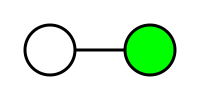
\includegraphics[height=\baselineskip]{img/subgraph/wg.png}}を \\
	\vspace{-60px}
	\begin{columns}[t]
		\begin{column}{0.50\hsize}
			\begin{tcolorbox}[colback=white]
				含まない \\
				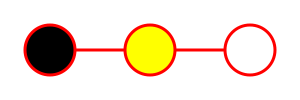
\includegraphics[height=1\baselineskip]{img/graph/g02r.png} \hspace{30px}
				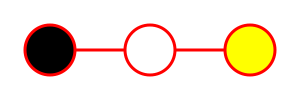
\includegraphics[height=1\baselineskip]{img/graph/g03r.png} \\
				\vspace{10px} \\
				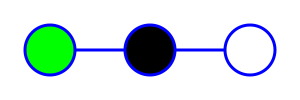
\includegraphics[height=1\baselineskip]{img/graph/g04b.png} \\
			\end{tcolorbox}
		\end{column}
		\begin{column}{0.50\hsize}
			\begin{tcolorbox}[colback=white]
				含む \\
				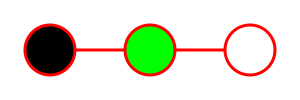
\includegraphics[height=1\baselineskip]{img/graph/g01r.png} \hspace{30px}
				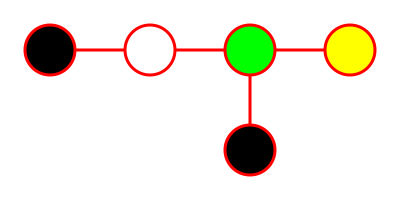
\includegraphics[height=2\baselineskip]{img/graph/g07r.png} \\
				\vspace{10px} \\
				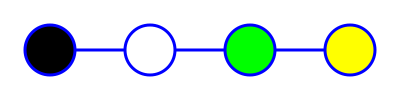
\includegraphics[height=1\baselineskip]{img/graph/g08b.png}
				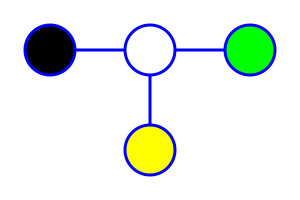
\includegraphics[height=2\baselineskip]{img/graph/g05b.png}
				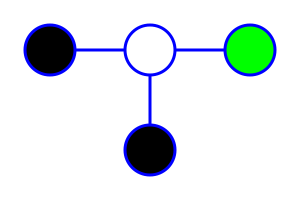
\includegraphics[height=2\baselineskip]{img/graph/g06b.png}
			\end{tcolorbox}
		\end{column}
	\end{columns}

	\vspace{60px}
	ここまで分かっているとき、 \\
	\raisebox{-10pt}{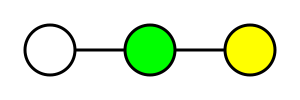
\includegraphics[height=\baselineskip]{img/subgraph/wgy.png}}の有無で分割することを考える \\

	理想の分割($\plus$のみ含む) \\
	\vspace{-60px}
	\begin{columns}[t]
		\begin{column}{0.50\hsize}
		\begin{tcolorbox}[colback=white]
			含まない \\
			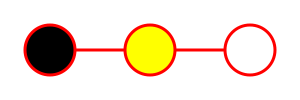
\includegraphics[height=0.7\baselineskip]{img/graph/g02r.png} \hspace{30px}
			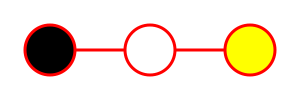
\includegraphics[height=0.7\baselineskip]{img/graph/g03r.png} \\
			\vspace{10px} \\
			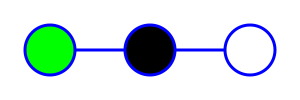
\includegraphics[height=0.7\baselineskip]{img/graph/g04b.png} \hspace{10px}
			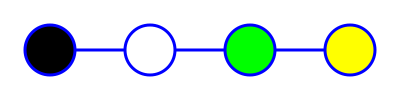
\includegraphics[height=0.7\baselineskip]{img/graph/g08b.png} \hspace{10px}
			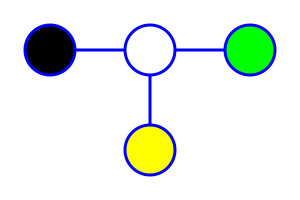
\includegraphics[height=1.4\baselineskip]{img/graph/g05b.png} \hspace{10px}
			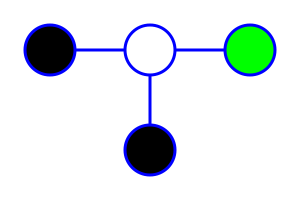
\includegraphics[height=1.4\baselineskip]{img/graph/g06b.png}
		\end{tcolorbox}
		\end{column}
		\begin{column}{0.50\hsize}
		\begin{tcolorbox}[colback=white,colframe=red]
			含む \\
			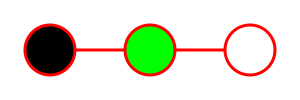
\includegraphics[height=0.7\baselineskip]{img/graph/g01r.png} \hspace{30px}
			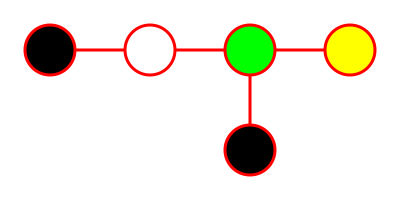
\includegraphics[height=1.4\baselineskip]{img/graph/g07r.png} \\
		\end{tcolorbox}
		\end{column}
	\end{columns}

	\vspace{50px}

	理想の分割($\minus$のみ含む) \\
	\vspace{-60px}
	\begin{columns}[t]
		\begin{column}{0.50\hsize}
		\begin{tcolorbox}[colback=white]
			含まない \\
			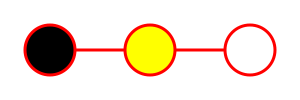
\includegraphics[height=0.7\baselineskip]{img/graph/g02r.png} \hspace{30px}
			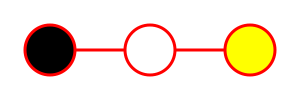
\includegraphics[height=0.7\baselineskip]{img/graph/g03r.png} \\
			\vspace{10px} \\
			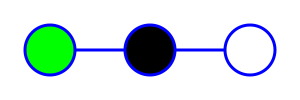
\includegraphics[height=0.7\baselineskip]{img/graph/g04b.png} \hspace{30px}
			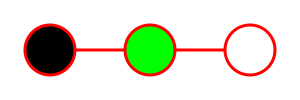
\includegraphics[height=0.7\baselineskip]{img/graph/g01r.png} \hspace{30px}
			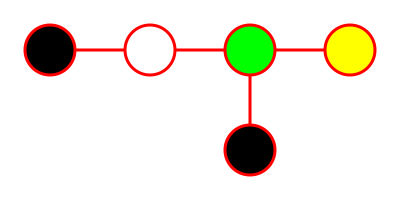
\includegraphics[height=1.4\baselineskip]{img/graph/g07r.png} \\
		\end{tcolorbox}
		\end{column}
		\begin{column}{0.50\hsize}
		\begin{tcolorbox}[colback=white,colframe=blue]
			含む \\
			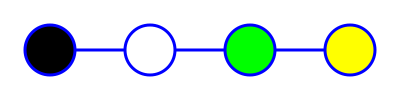
\includegraphics[height=0.7\baselineskip]{img/graph/g08b.png}
			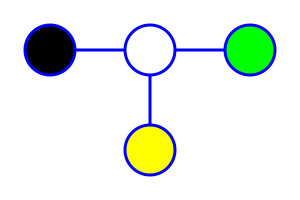
\includegraphics[height=1.4\baselineskip]{img/graph/g05b.png}
			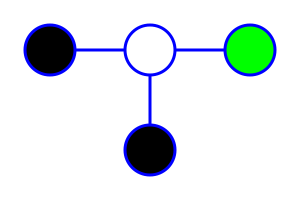
\includegraphics[height=1.4\baselineskip]{img/graph/g06b.png}
		\end{tcolorbox}
		\end{column}
	\end{columns}



\end{tcolorbox}
